% arara: xelatex
% arara: xelatex
% arara: xelatex


% options:
% thesis=B bachelor's thesis
% thesis=M master's thesis
% czech thesis in Czech language
% english thesis in English language
% hidelinks remove colour boxes around hyperlinks

\documentclass[thesis=B,english]{FITthesis}[2012/10/20]

% \usepackage[utf8]{inputenc} % LaTeX source encoded as UTF-8
% \usepackage[latin2]{inputenc} % LaTeX source encoded as ISO-8859-2
% \usepackage[cp1250]{inputenc} % LaTeX source encoded as Windows-1250

\usepackage{graphicx} %graphics files inclusion
\usepackage{float}
\usepackage{csquotes}
% \usepackage{subfig} %subfigures
% \usepackage{amsmath} %advanced maths
% \usepackage{amssymb} %additional math symbols
\usepackage{dirtree} %directory tree visualisation

% % list of acronyms
% \usepackage[acronym,nonumberlist,toc,numberedsection=autolabel]{glossaries}
% \iflanguage{czech}{\renewcommand*{\acronymname}{Seznam pou{\v z}it{\' y}ch zkratek}}{}
% \makeglossaries

% % % % % % % % % % % % % % % % % % % % % % % % % % % % % % 
% EDIT THIS
% % % % % % % % % % % % % % % % % % % % % % % % % % % % % % 

\department{Department of Software Engeeniring}
\title{StudyPad - Android Client}
\newcommand{\appname}{StudyPad}
\authorGN{Roman} %author's given name/names
\authorFN{Levinzon} %author's surname
\author{Roman Levinzon} %author's name without academic degrees
\authorWithDegrees{Roman Levinzon} %author's name with academic degrees
\supervisor{Ing. Miroslav Bal{\'i}k, Ph.D}
\acknowledgements{THANKS (remove entirely in case you do not with to thank anyone)}
\abstractEN{StudyPad is a combination of note-taking service and a social network, aimed to help students to memorise different pieces of information.  The goal of this thesis is to develop an application for Android OS which will serve as client. This text acknowledges existing solutions, contains domain and requirements analysis, description and choise of application's architecture and it's implementation}


\abstractCS{StudyPad je kombinace slu{\v z}by pro pori{\v z}ovan{\' i} pozn{\'a}mek a soc{\'i}{\'a}ln{\'i} s{\'i}t{\v e} s c{\'i}lem  pomoci studentum zapamatovat si ruzn{\'e} informace. C{\'i}lem pr{\'a}ce je vyvinout aplikaci pro OS Android, kter{\'a} bude slou{\v z}it jako klient. Tento text uzn{\'a}v{\'a} st{\'a}vaj{\' i}c{\'i} {\v r}e{\v s}en{\'i}, obsahuje anal{\'y}zu dom{\'e}n a po{\v z}adavku, popis a v{\'y}b{\v e}r architektury aplikace a jej{\'i} implementace}
\placeForDeclarationOfAuthenticity{Prague}
\keywordsCS{Android, Kotlin, MVVM}
\keywordsEN{Android, Kotlin, MVVM}
\declarationOfAuthenticityOption{1} %select as appropriate, according to the desired license (integer 1-6)
% \website{http://site.example/thesis} %optional thesis URL


\begin{document}

% \newacronym{CVUT}{{\v C}VUT}{{\v C}esk{\' e} vysok{\' e} u{\v c}en{\' i} technick{\' e} v Praze}
% \newacronym{FIT}{FIT}{Fakulta informa{\v c}n{\' i}ch technologi{\' i}}

\setsecnumdepth{part}
\chapter{Introduction}

Each year, our smartphones get smarter and mobile applications -- more advanced. Arrival of smartphones and mobile applications completely changed our way of living, made it easier, and it is hard to come up with the single aspect of life, which has not been improved by one or the other application. They are everywhere: helping us to navigate in our neighbourhood, keeping us up to date with latest news, helping us to stay in touch with our loved ones, stay  fit and healthy and more. And some of the most popular applications tend to teach us something new.	

Educational apps are one of the most popular apps on both mobile platforms (iOS and Android). Many of them use flash card system in the study process -- displaying small pieces of information one after another, so the user could memorise it more easily. However, most of these services are fairly limited in terms of what they are trying to teach and some of the greatest  features are scattered across different applications and services. \appname\ wants to give its users freedom in what they could learn, and give them proper tools to collaborate on study materials to make their education process even more easier.

\subsection{\appname\ service}
\appname\ is a combination of a note taking service and a social network. It is intended for students and everyone who wishes to learn something new. \appname\ primary focus is on the content creation, its sharing and discovery.

\appname\ core concepts are \textit{Notebooks} and \textit{Notes}. Notebook is simply a collection of notes united by one theme. This may be a subject in school, a language that you would like to learn, or a set of questions that you could hear at a job interview. Note, in turn, is a part of the notebook and represents a single piece information that has a name and a content. It can also be interpreted as a question and answer, or a term and its definition.
\\

Each user has his/her own space where he can create, store and edit notebooks and notes (hereafter \textit{Library}). All notebooks stored in the library can be used in various tests and exercises to help users to memorise its content. 

\appname\ also allows users to easily share these notebooks with each other. Each notebook can be shared by creating a published version of it (hereafter Published Notebook),thereby making it available to everyone else for viewing and importing.
The publication process involves providing additional information about the notebook, including its name, optional description, topic and optional tags, that serve to narrow the topic. All this data along with Author's school and language will then be used in the process of searching and filtering - which will facilitate the search for the necessary materials. There is also a functionality to quickly share a notebook by sending a link, which will act as a deep-link, navigating user directly to a Published Notebook.

The Author of the notebook reserves the right to make edits/corrections to the Published Notebook. Other users (hereinafter subscribers) in turn can save a Published Notebook to their library, or suggest the author changes/corrections to improve the content inside. By saving Published notebook to his/her library, subscriber will be able to make any local changes as he sees fit and use it as normal. Subscriber will be notified about any updates to the Published Notebook so that they can apply changes to their local versions, however, any local changes made by him/her will be deleted. The author of the notebook, in turn, will be notified about latest suggestions and comments left by subscribers

\setsecnumdepth{all}
\chapter{Analysis}
This chapter contains \appname\ system description and analysis with the goal to identify requirements and how it is compared with its rivals


\section{System description}

\appname\ system follows classic client-server software architecture. Server part is represented by Spring Boot application, which is communicating with it clients using REST API. Client part consists of client applications for several platforms: Android, iOS and Web. Web client is being developed alongside the Android one to serve as an Admin Panel. Main task of this thesis is to deliver an Android client.

The detailed structure of the Android client structure and how it is connected with other components is presented on the component diagram on figure \ref{fig:deploy}. 

 Android component will be divided into three layers: Data layer, Domain Layer and Presentation layer. Data layer is only responsible for downloading and storing data. Business layer responsibility is to handle user interactions and converting downloaded data to something that presentation layer can present. Presentation layer is only responsible for displaying data. Android component will be also connected to Facebook SDK, Google Auth SDK and Firebase Sdk to provide authentication options. Firebase SDK will also enable analytics service, crash reporting and push notifications.
\newpage
\begin{figure}[H]
  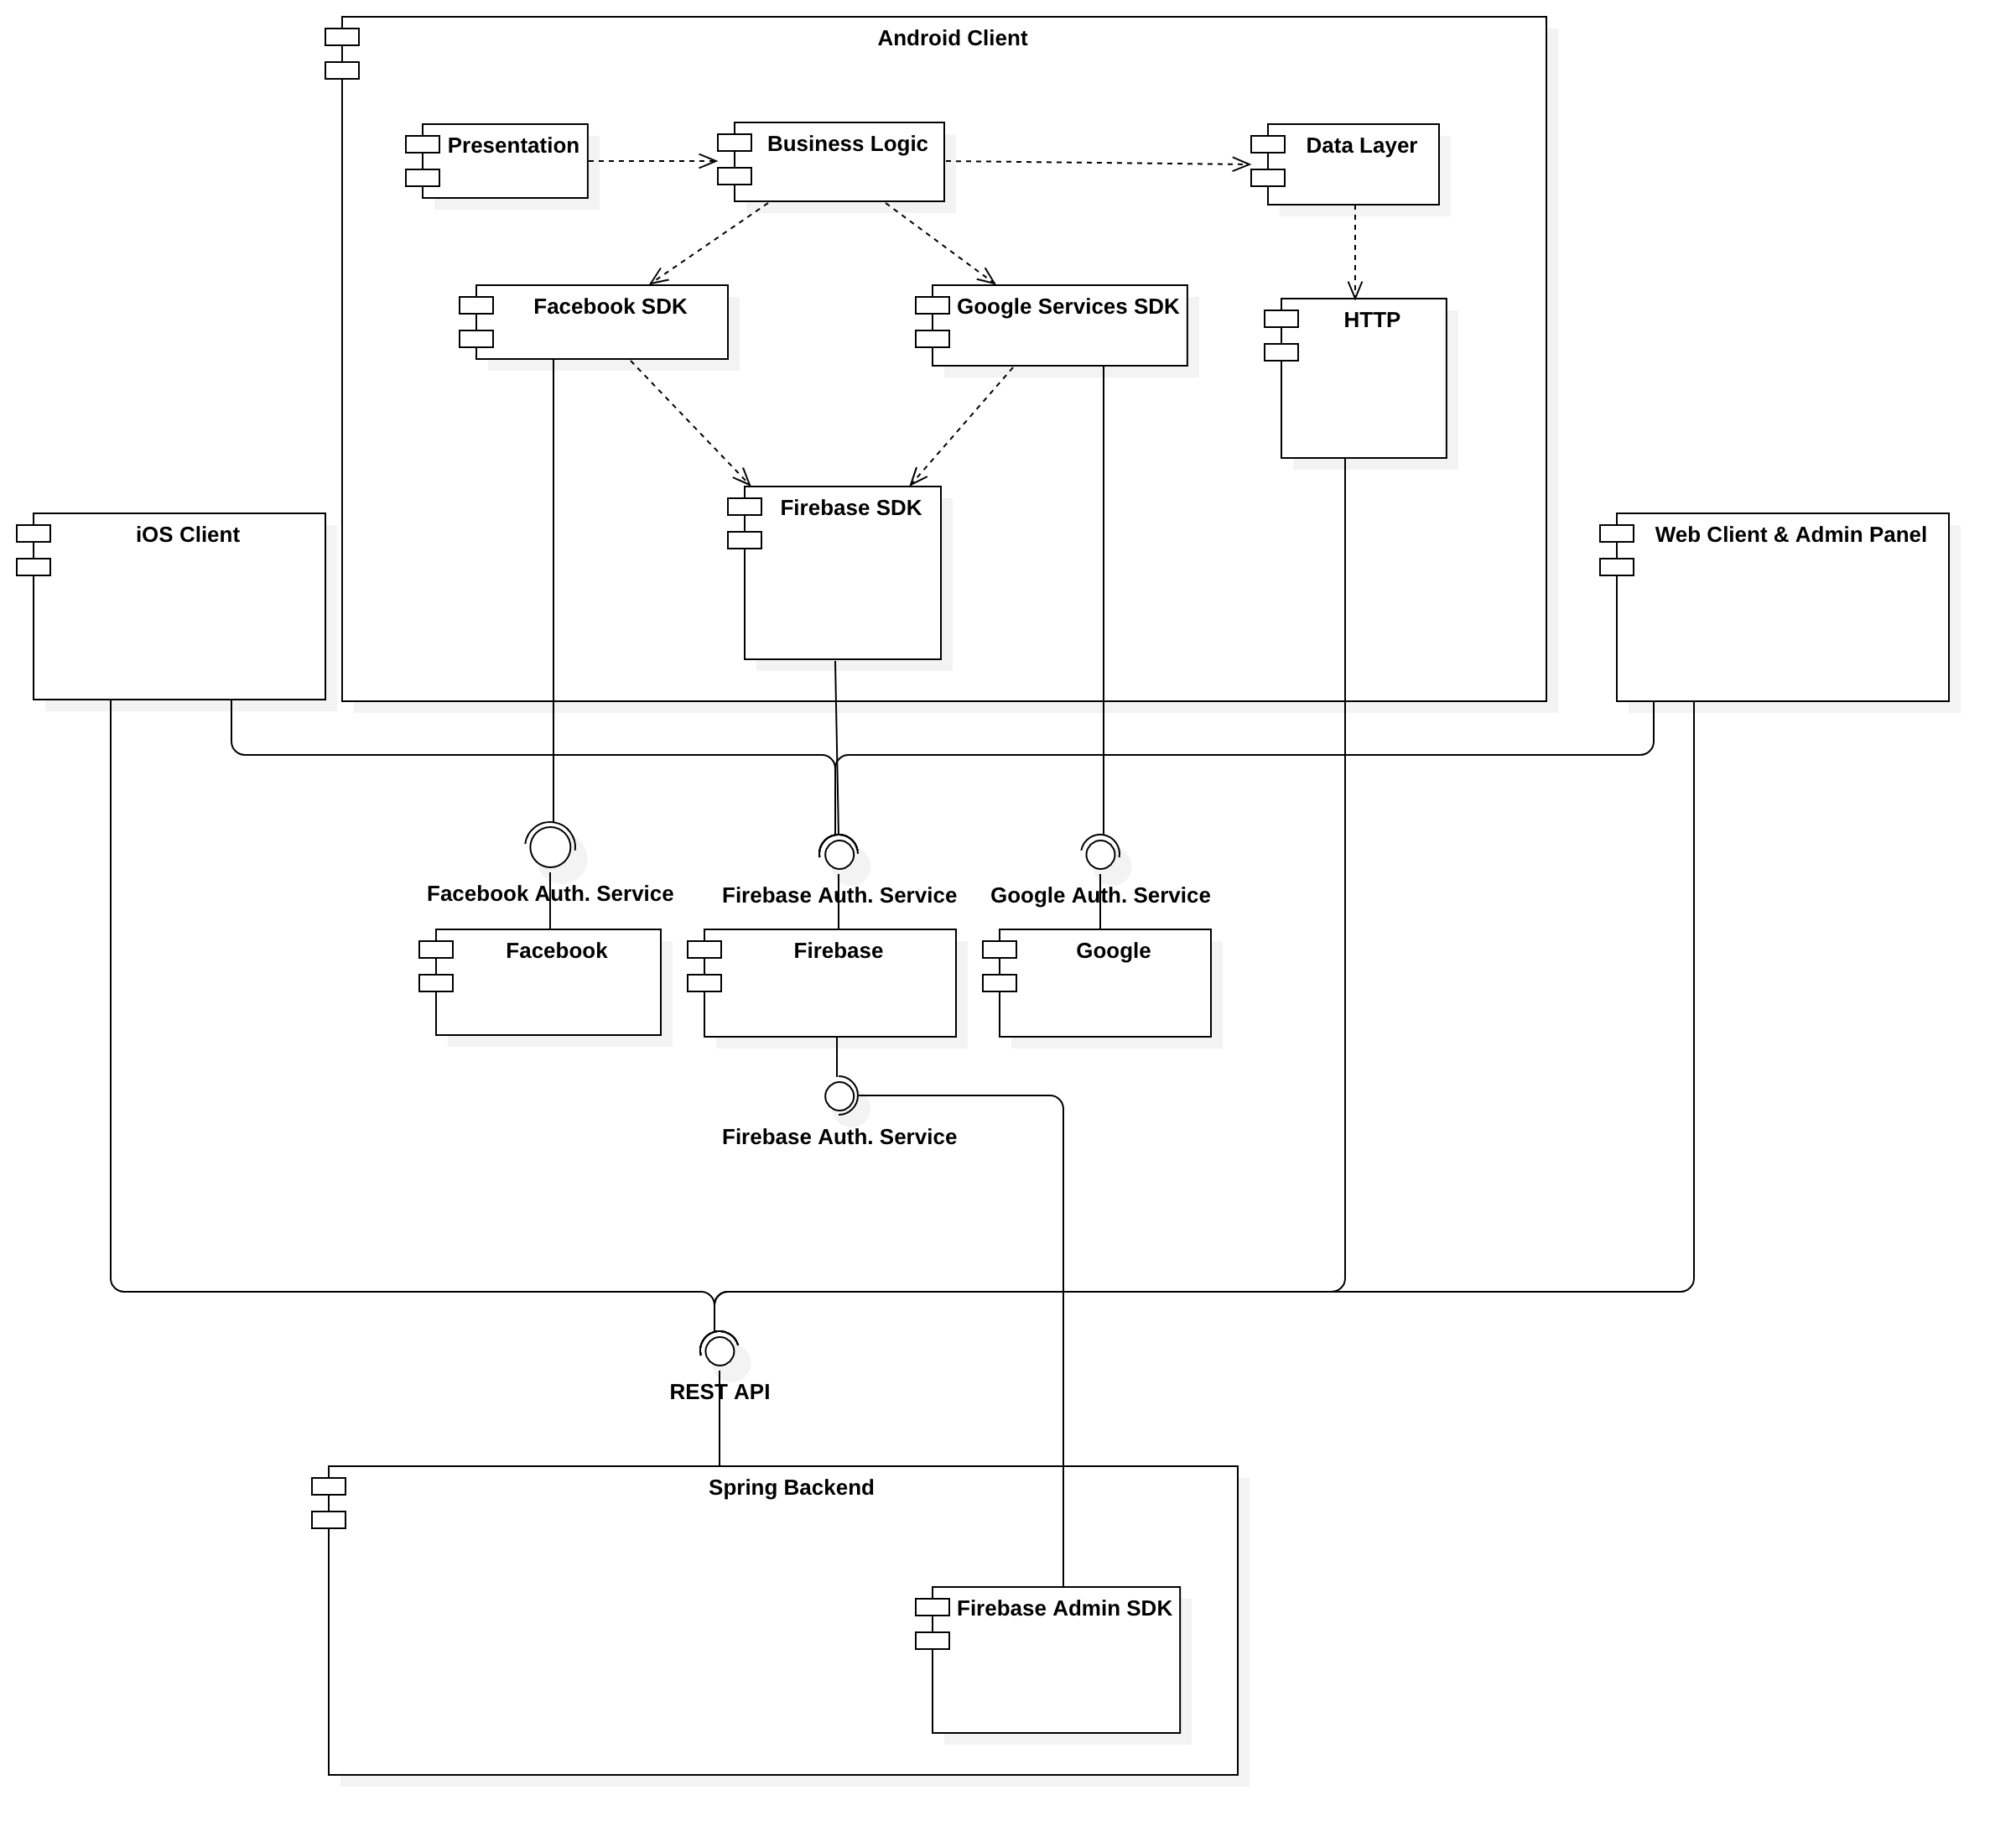
\includegraphics[scale=0.4]{deployment}
  \caption{Component Diagram}
  \label{fig:deploy}
\end{figure}


\newpage
\section{Domain Description}
 Class Diagram on figure \ref{fig:domain} represents Domain Model of the application, it provides visual representation of Entities and relations between them. Design is based on the entities used on server-side

\begin{figure}[H]
  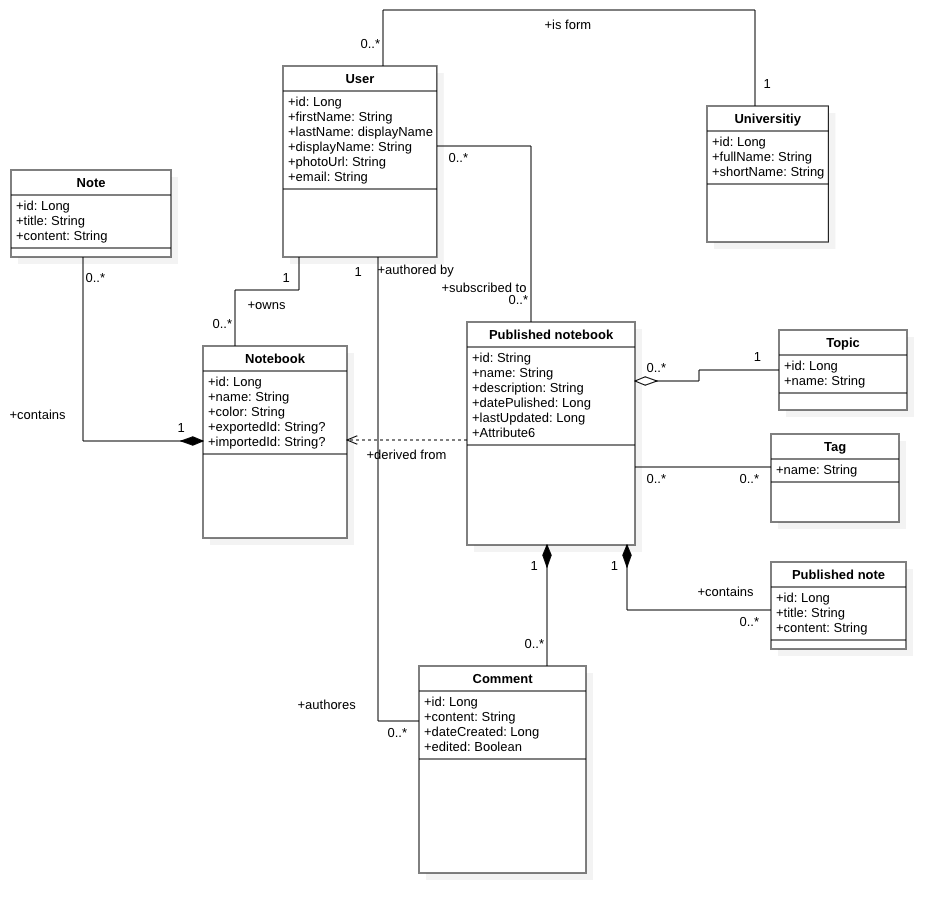
\includegraphics[width=\linewidth]{Domain}
  \caption{Domain Diagram}
  \label{fig:domain}
\end{figure}

 

\subsection{User}
	User entity represents someone who have completed registration flow using one of the client applications. This entity contains such properties as: firstName, lastName, email, password, university. Due to the fact, that \appname\ provides several ways for user to authorise, some of the properties will either come from the user's input or from the 3d party API (such as Firebase)

	
\subsection{Note}
	Note represents a single piece of information. It consists of two properties: title and content. These can be described as term and definition or question and answer. Every note must be assigned to one of the notebooks, hence theres a 1:N relation
\subsection{Notebook}
	Notebook is one of the main entities used in the application flow, and  can be created by an authenticated user. Soul purpose of the Notebook is to store Notes and serve as a source for Published Notebook. Properties name and color are used to help users distinct between different Notebooks
	
	
\subsection{University}
University represents school, where User can assign himself as a student during registration flow. It is used to unite users from the same school to make content searching easier. 

\subsection{Published Notebook}
Published Notebook represents a shareable content. It can be created by user, based on one of his/her notebooks by providing some additional details:
name, optional description,  topic and optional list of tags. All these details are later used in a searching flow to optimise results.

\subsection{Published Note}
Published Note represent the note inside of the Published Notebook and contains the exact same properties as usual note

\subsection{Topic}
Topic represents main topic or subject of the Published Notebook. Topic consist of only one property -- its name
\subsection{Tag}
Tag is a short label thats attached to the Published Notebook. It is mainly  used to narrow the topic or school. Tag has only one property -- its actual value stored as name

\subsection{Comment}
Users can comment on published notebooks. Most of the properties are assigned automatically, the only exception is content which is property that represents the body of the comment.

\section{Android Platform}




\newpage
\section{Requirements}
It is important to establish all functional and non-functional requirements for \appname. Section bellow contains all requirements designed before the start
of the development

\subsection{Functional requirements}
\bigskip
\textbf{User Authentication}
\begin{itemize}
	\item \textbf{F1: Registration/Login using email} Access to \appname\ is possible by creating an account using email address/password combination.
	\item \textbf{F2: Registration/Login using Facebook} User will be able to use his/her Facebook account to access \appname.
	\item \textbf{F3: Registration/Login using Google} User will be able to use his/her Google account to access \appname.
	\item \textbf{F4: Store OAuth token} API Authentication Token will be stored in device memory.
	\item \textbf{F5: Token refreshment} API Token will be refreshed when needed, so user won't have to login again.
	\item \textbf{F6: University selection} As a part of user registration flow, user will be able to select his/her university.
	\item \textbf{F7: University Addition} User will be able to add his/her school, in case of not finding it in \appname\ database.
\end{itemize}
\bigskip
\textbf{Library Management (Notes \& Notebooks)}
\begin{itemize}
	\item \textbf{F7: Notebook creation} User will be able to create new notebooks with the name he/she choose.
	\item \textbf{F8: Notebook deletion} User will be able to delete existing notebooks.
	\item \textbf{F9: Notebook name edition} User will be able to edit notebooks names.
	\item \textbf{F10: Note creation} User will be able to create a note with specific title and content.
	\item \textbf{F11: Note edition} User will be able to edit existing note, or completely delete it.
	\item \textbf{F12: Show Notebooks} : User will be able to view all the notebooks he/she created.
	\item \textbf{F13: Show Notes}: By clicking on notebook item, user will be able to view the list of notes that are assigned to this notebook.
	\item \textbf{F14: MathJax support}: User will be able to use complex mathematical expressions as notes content
\end{itemize}

\bigskip
\textbf{Sharing Hub}
\begin{itemize}
	\item \textbf{F15: View published notebooks} User will be able to view notebooks published by other users.
	\item \textbf{F16: Search through published books} User will be able to search through the published notebooks by applying different filters (such as author, university and subject/topic).
	\item \textbf{F17: Browse through published notebook} User will be able to see notes inside the notebook that's been published.
	\item \textbf{F18: View comments} User will be able to view others users comments discussing a notebook that's been published.
	\item \textbf{F19: Leave a comment} User can comment on other user published notebook.
	\item \textbf{F20: Delete a comment} Application will let user to delete his/her comment.
	\item \textbf{F21: Save published notebook} User will be able to save published notebook to his/her library.
	\item \textbf{F22: Publish notebook} User will be able to publish his/her notebook.
	\item \textbf{F23: Update published notebook} Author of the published notebook will be able to update its information.
	\item \textbf{F24: Delete published notebook} Author of the published notebook will be able to delete the his/her notebook from shared space.
	\item \textbf{F25: Share notebook} User will be able to share his/her notebook by generating a deep-link.
	\item \textbf{F26: Notification on update:q} User will be notified on updates to the Published notebook he subscribed to
	\item \textbf{F27: Suggestions} Subscribers will be able to suggest a change or correction to the Published Notebook
	\item \textbf{F28: Copy Published Notebook} User will be able to copy published notebook. This will 
 \end{itemize}

\bigskip
\textbf{Study Hub}
\begin{itemize}
	\item \textbf{F29: Start a basic self-check} User will be able to use an interactive way to look through his/her notes
	\item \textbf{F30: Start a written test} User will be able to participate in a written test based on one of notebooks to test his/her knowledge
	\item \textbf{F31: Start a quiz} User will be able to participate in quiz challenge that will be based on one of his/her notebooks
	
\end{itemize}


\bigskip
\textbf{Settings}
\begin{itemize}
	\item \textbf{F32: View Profile Information} User will be able to view his/her profile information such as first name, last name and  university.
	\item \textbf{F33: Edit Profile Information} User will be able to edit his/her profile information.
	\item \textbf{F34: Logout} User will be able to logout from the application.
\end{itemize}


\subsection{Non-functional requirements}

\begin{itemize}
  \item \textbf{N1: Native Android application}  Application will be written using native Android SDK.
  \item \textbf{N2: Android Version} Application minimal SDK version must be low enough to support as many devices as possible and high enough to use most applicable  Android APIs considering other functional and non-functional requirements.
  \item \textbf{N3: Material Design} Application user interface will follow latest Material design guidelines and best practises.
  \item \textbf{N4: Scalable app architecture} Application's architecture must be scalable and easy testable.
  \item \textbf{N5: Tablet \& Phone support} Application GUI must be well suited for multiple screen sizes.
  \item \textbf{N6: App Localisation} Application will be able to adapt to different languages based on user locale
\end{itemize}


\newpage

\section{Existing solutions}

There are several services out there, whose goal is similar to \appname. However, most of the solutions are limited to learning languages and have limited sharing and/or searching options. 

\subsection{StudyBlue overview}

\textbf{StudyBlue} not only partially shares a name with \appname\ but also a goal and a wide set of features. It is clearly on of the biggest rivals on the market and it is very important to determine what StudyBlue does right and what not.

Notebooks here are called \textit{decks} and notes are represented by \textit{cards}. Moreover, all decks in StudyBlue are stored in specialised folders named Classes and Interests. Interest, as an entity, not only stores decks, but also unites them by a subject or a topic (eg Spanish, Literature). Being a student of the university, user can also create an interest, that will be connected to his/her school -- Class. Both Interests and Classes are split into 2 parts, shared space, where user can found all the decks created by other users, and personal space, where user can keep decks he/she created, saved or copied.


\begin{itemize}
	\item \textbf{Library management:} Main difference in library management comes with the fact, that each deck must be associated with an Interest or Class, moreover, it's not possible just to create deck, user have to create at least 2 cards first. Every  Class or an Interest, user adds, is being stored in a \textit{Backpack}. So, Backpack here acts as a personal library, and serves as an entry point for all the decks user have saved. 
	\item \textbf{Importing}: As mentioned before, user can save deck from an existing shared folder to his personal folder, but he would not be able to make any editions unless he made a copy.
	\item \textbf{Discovering:} The fact that all decks are either assigned to an Interest or a Class makes searching quite simple. User can search for deck, classes and users by its name.All these searching options are separated in the UI, so there is no way of combining them. To search for the decks based on the Interest, user have to add this Interest to his/her \enquote{Backpack}
	\item \textbf{UI \&  UX}: StudyBlue has been in development roughly since 2009, and is for now, UI looks outdated and UX can be greatly improved just by applying best practises. Confusing UI elements, inconsistent 
\end{itemize}

 \subsection{Quzlet overview}
\textbf{Quizlet} is primarily used for learning languages, from where most of the limitations come from. Closest analogy to Notebook there is Study set with Terms inside. This makes it easier for tests generation, but limits user when he/she is trying to learn anything other than new words



\begin{itemize}
	\item \textbf{Publishing}: Content publishing process is very different to what \appname\ is trying to achieve. All study sets are visible to other users by default, which makes it hard, if not impossible, to distinct between local and shared published set.
	\item \textbf{Importing}: Importing flow allows user to either copy or save study set to a specific folder. This flow may confuse some of the users, because only copy allows actually add a study set to user library and modify it. Saving study set to the specific folder only saves the link to it and splits library management in 2 parts.
	\item \textbf{Discovering:} This limitation comes from the fact, that Quizlet is an app for studying new languages. As a consequence, the only distinctions between Study sets are its name and a language. These are the only 2 options available for when searching through published study sets.

\end{itemize}

\subsection{Cram overview}
\textbf{Cram} is very similar to Quizlet but seems much more outdated in terms of UX and brings some sharing limitations to the table.

\begin{itemize}
	\item  \textbf{Publishing:} Content publishing is similar to Quizlet - All sets are either visible by other users or not. Sharing a deep-link to a single study set was not functional at the time of writing this section
	\item \textbf{Discovering} Searching for content in Cram is even more limited comparing to Quizlet, only name of the study set is used
	\item \textbf{Importing} Library management here is split in 3 parts: User personal sets, Favourite sets, and Recently studied. When searching, there is no way to save published study set to personal library, however, it will be automatically saved to Recent section, or user can add it manually to Favourites. This makes it impossible to make local edits
\end{itemize}

\subsection{TinyCards overview}

\textbf{TinyCards} is an application made by Duolingo, one of the biggest app for learning languages. TinyCard is meant to be more generic as it offers users to create custom study sets, often not limited to languages
	\begin{itemize}
		\item \textbf{Importing:} Similar to Cram, it is not possible to edit the study set user have downloaded and saved to his library
		\item \textbf{Challenges:} Tests for user are generated automatically and there is no way to choose test type
	\end{itemize}
	
\newpage

\chapter{Design}
\section{Wireframes}
\section{Application architecture}
\section{Platform-specific model}
\section{Main sequence diagrams}

\chapter{Implementation}
\section{Choice of technologies}
\section{Component diagram}
\section{Installation}


\chapter{Testing}


\setsecnumdepth{part}
\chapter{Conclusion}


\bibliographystyle{iso690}
\bibliography{mybibliographyfile}

\setsecnumdepth{all}
\appendix

\chapter{Acronyms}
% \printglossaries
\begin{description}
	\item[GUI] Graphical user interface
	\item[XML] Extensible markup language
\end{description}


\chapter{Contents of enclosed CD}

%change appropriately

\begin{figure}
	\dirtree{%
		.1 readme.txt\DTcomment{the file with CD contents description}.
		.1 exe\DTcomment{the directory with executables}.
		.1 src\DTcomment{the directory of source codes}.
		.2 wbdcm\DTcomment{implementation sources}.
		.2 thesis\DTcomment{the directory of \LaTeX{} source codes of the thesis}.
		.1 text\DTcomment{the thesis text directory}.
		.2 thesis.pdf\DTcomment{the thesis text in PDF format}.
		.2 thesis.ps\DTcomment{the thesis text in PS format}.
	}
\end{figure}

\end{document}
